\chapter{Time-memory-data tradeoff using Rainbow tables}
\label{chapter:tmdto-rainbow}

\paragraph{Summary}


\section{Rainbow table for block ciphers}
\label{sec:rainbow-block}

Rainbow table was introduced by Philippe Oechslin in \cite{oechslin:mfc}. Rainbow table (or rainbow chains, as called by the author) is a different way of precomputing data for the attack phase of a TMTO attack. Oechslin introduced rainbow table on block ciphers with improvements over the Hellman tables. By using rainbow table, the attack time is supposed to be reduced by a factor of $2$.

In Hellman tables, merging of chains within different tables is prevented by using different reduction functions for each table. However, collisions within the same table cannot be avoided completely. Though the number of elements in each table is restricted according to the relation derived using the variant of the birthday paradox, still no guarantee can be provided that collisions would not occur in the same table. This is due to the fact that the relation is probabilistic in nature, as is the birthday paradox from which it is derived. Rainbow table reduces the problem of collisions considerably.\\

\noindent \textit{\textbf{Precomputation phase.}} The rainbow table comprises of one huge table instead of $t$ tables, with $mt$ chains each having $t$ keys. The interesting difference from Hellman tables is that instead of reduction functions being changed for tables, reduction function are changed by column. If $SP_i$ is the starting point of a chain, then subsequent keys are computed by the functions \mbox{$F_1, F_2, \cdots, F_t$}, where $F_j(K) = R_j(E_{K}(P))$ for $1 \leq j \leq t$. This is shown in the following equations. 

\begin{align*}
& & K_{i,0} & = SP_i & & & &\\
1&. &K_{i,1} & = F_1(K_{i,0}) & & & &\\
2&. &K_{i,2} & = F_2(K_{i,1}) & & & &\\
& & &\vdots & & & &\\
(t-1)&. &K_{i,t-1} & = F_{t-1}(K_{i,t-2}) & & & &\\
(t)&. &K_{i,t} & = F_t(K_{i,t-1}) & & & &\\
& & EP_i & = K_{i,t} & & & &\\
\end{align*}

For every chain, the same sequence of mapping functions from $F_1$ to $F_t$ are used in computing subsequent keys. As usual, the starting and end points for each chain are stored in a hashtable, with the end points as the hash key and the starting points as the hash value. A rainbow table is shown in figure \ref{fig:rainbow-table}.

\begin{figure}[ht!]
	\centering
		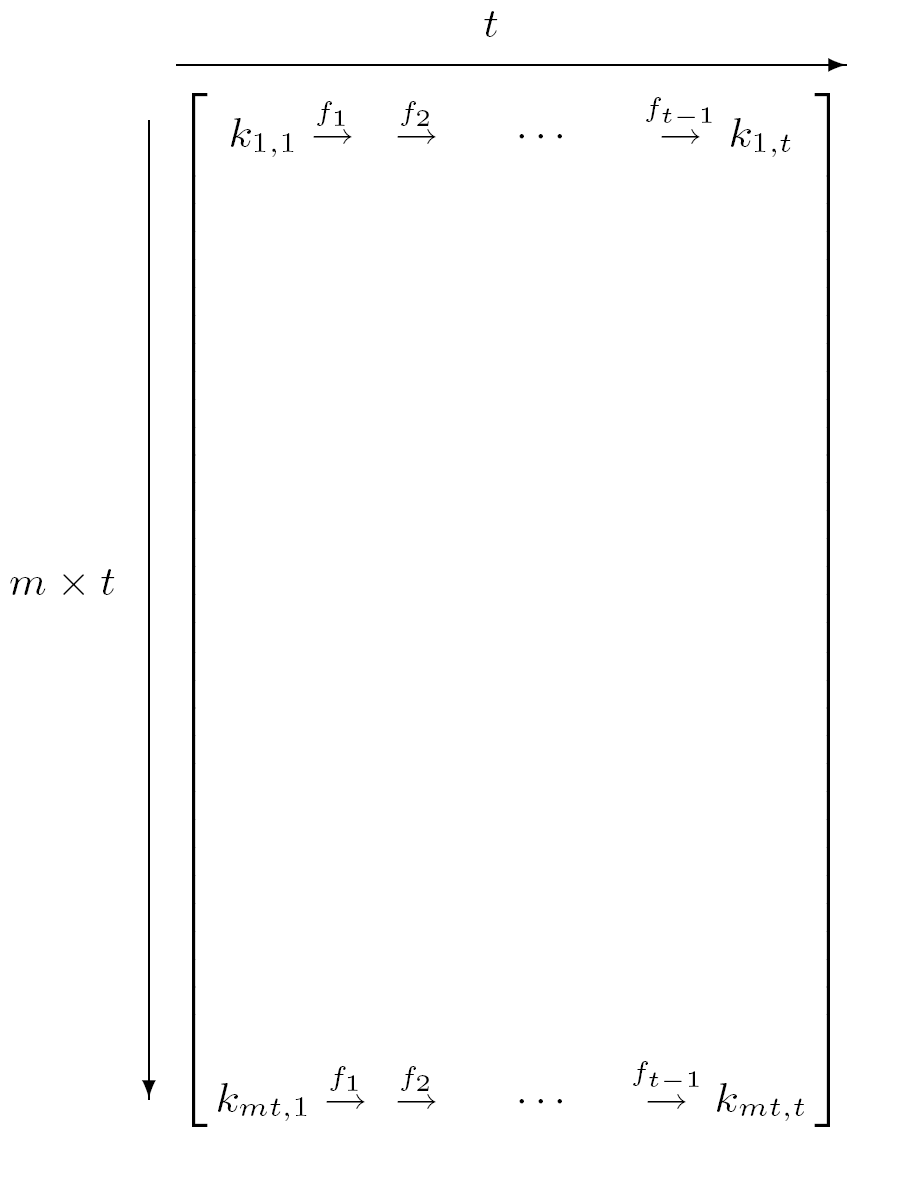
\includegraphics[width=3.5in]{./figures/rainbow-table.PNG}
	\caption{Rainbow table for block ciphers}	
	\label{fig:rainbow-table}
\end{figure}

The time for preparing the rainbow table is the same as the number of computations carried out. This is equal to $P$ = $mt \times t$ = $mt^2$. Also, the order of memory required for the hash table is $M$ = $mt$. \\

\noindent \textit{\textbf{Attack phase.}} The attack phase is a little more complicated as compared to that for Hellman tables. But, as we shall see, the number of computations required in the worst case, to find a match, is reduced by a factor of $2$. 

First, let's consider the possibility of the ciphertext appearing in the last column of the rainbow table. If this is the case, then an end point $EP_i$ would match with the reduction of the ciphertext $C$ which is $X$ = $R_t(C)$. Note that the reduction function for the $t$'th column is used here. If the match occurs, then $(t-1)$ computations are performed starting from the corresponding starting point $SP_i$, with the mapping function changing in each column. $K_{i,t-1}$ is then the required key, if it is not a false alarm. If the match does not occur, the number of operations (number of calls to any of the mapping functions $F_1$ to $F_t$) performed is $0$. 

So next, the possibility of $C$ appearing in the $(t-1)$'th column is explored. For this the value $X = F_{t}(R_{t-1}(C))$ is compared with the end points. If there is a match, then $(t-2)$ computations are performed from $SP_{i}$ using the mapping functions $F_1, F_2, \cdots, F_{t-2}$. The key $K_{i,t-2}$ computed is the required key. Otherwise, if there is no match, the number of operations performed is $1$.

This procedure is repeated for all the columns, until in a worst case scenario, $C$ happens to appear in the second column of the table. In such a case, we would iteratively call the mapping functions $F_2, F_3, \cdots, F_t$, thus amounting to $(t-1)$ operations, before $EP_j$ is matched. The total number of operations in the worst case scenario become, 

\begin{align*}
&= 0 + 1 + 2 + \cdots + (t-1)\\
&= t(t-1)/2\\
&\approx t^2/2
\end{align*}

The attack time then is of the order of $t^2/2$, thus $T$ = $t^2/2$.\\


\noindent \textit{\textbf{Tradeoff equation.}} Using the following equations, the tradeoff equation can be derived. 

\begin{align*}
M &= mt\\
T &= t^2/2\\
mt^2 &= N\\
\end{align*}
The tradeoff equation then comes to be,
\begin{align}
\label{eq:tmdto-rainbow-block} 2TM^2 &= N^2
\end{align}


\section{Rainbow tables for stream ciphers}
\label{sec:rainbow-stream}


\section{Results of implementation}
\label{sec:rainbow-impl}